\documentclass[12pt,a4paper]{article}

\usepackage{borochkin_article}

\begin{document}
\section{Нормальное распределение}
\small
Значения, приведенные в таблице, представляют собой величину площади под  стандартной нормальной (гауссовой) кривой от 0 до соответствующего z-значения. 
\begin{figure}[H]
\centering
	\begin{subfigure}[t]{6cm}
		\centering
		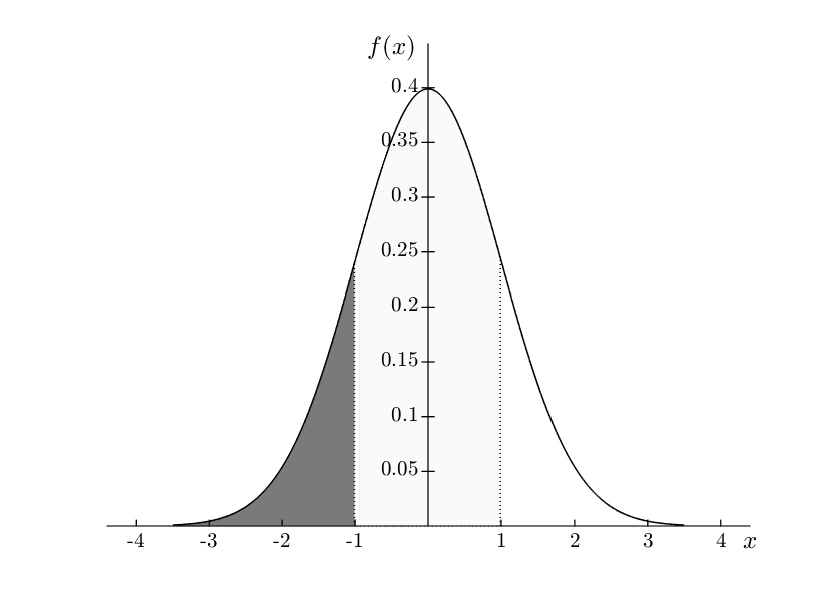
\includegraphics[scale=0.4]{img/normal_pdf.png}
		\caption{Плотность вероятности\\$f(x) = \frac{1}{\sqrt{2\pi} } \; e^{-\frac{x^2}{2}}$}
\label{fig:a_normal_pdf}	
	\end{subfigure}
	\begin{subfigure}[t]{7cm}
		\centering
		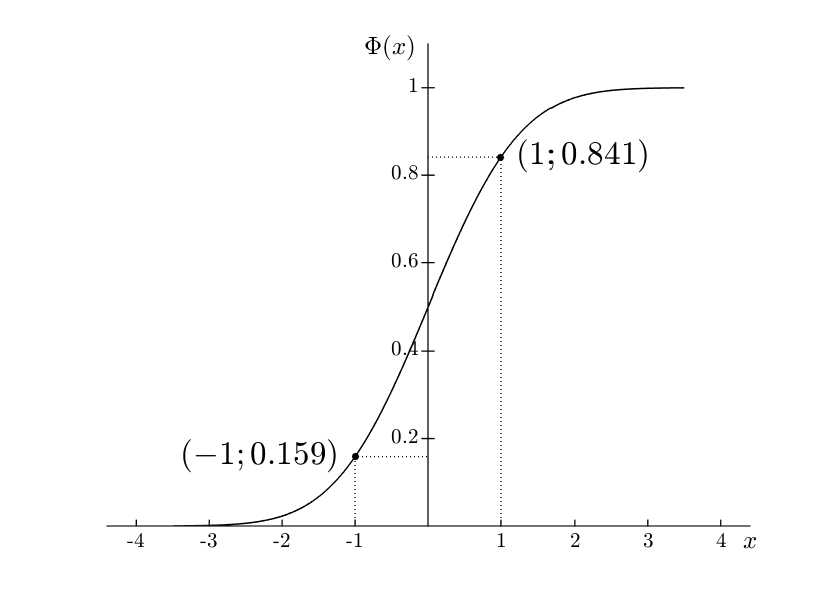
\includegraphics[scale=0.4]{img/normal_cdf.png}
		\caption{Кумулятивная функция\\$\Phi(x)\; = \;\frac{1}{\sqrt{2\pi}} \int_{-\infty}^x e^{-t^2/2} \, dt$}
\label{fig:b_normal_cdf}
	\end{subfigure}
	\caption{Графики функций стандартного нормального распределения}\label{fig:df_and_cdf}
\end{figure}

% Table generated by Excel2LaTeX from sheet 'норм'
\begin{table}[H]
  \fontsize{8pt}{8pt}\selectfont
  \centering
%  \caption{\parbox[t]{10cm}{Значения кумулятивной функции стандартного нормального распределения $\Phi(x)\; = \;\frac{1}{\sqrt{2\pi}} \int_{-\infty}^x e^{-t^2/2} \, dt$ }}
  \captionsetup{justification=centering}
  \caption{Кумулятивная функция стандартного нормального распределения}
    \begin{tabular}{rrrrrrrrrrr}
    \toprule
    x     & \multicolumn{1}{c}{           -     } & \multicolumn{1}{c}{       0,01   } & \multicolumn{1}{c}{       0,02   } & \multicolumn{1}{c}{       0,03   } & \multicolumn{1}{c}{       0,04   } & \multicolumn{1}{c}{       0,05   } & \multicolumn{1}{c}{       0,06   } & \multicolumn{1}{c}{       0,07   } & \multicolumn{1}{c}{       0,08   } & \multicolumn{1}{c}{       0,09   } \\
    \midrule
0     & 0,00000 & 0,00399 & 0,00798 & 0,01197 & 0,01595 & 0,01994 & 0,02392 & 0,02790 & 0,03188 & 0,03586 \\
    0,1   & 0,03983 & 0,04380 & 0,04776 & 0,05172 & 0,05567 & 0,05962 & 0,06356 & 0,06749 & 0,07142 & 0,07535 \\
    0,2   & 0,07926 & 0,08317 & 0,08706 & 0,09095 & 0,09483 & 0,09871 & 0,10257 & 0,10642 & 0,11026 & 0,11409 \\
    0,3   & 0,11791 & 0,12172 & 0,12552 & 0,12930 & 0,13307 & 0,13683 & 0,14058 & 0,14431 & 0,14803 & 0,15173 \\
    0,4   & 0,15542 & 0,15910 & 0,16276 & 0,16640 & 0,17003 & 0,17364 & 0,17724 & 0,18082 & 0,18439 & 0,18793 \\
    0,5   & 0,19146 & 0,19497 & 0,19847 & 0,20194 & 0,20540 & 0,20884 & 0,21226 & 0,21566 & 0,21904 & 0,22240 \\
    0,6   & 0,22575 & 0,22907 & 0,23237 & 0,23565 & 0,23891 & 0,24215 & 0,24537 & 0,24857 & 0,25175 & 0,25490 \\
    0,7   & 0,25804 & 0,26115 & 0,26424 & 0,26730 & 0,27035 & 0,27337 & 0,27637 & 0,27935 & 0,28230 & 0,28524 \\
    0,8   & 0,28814 & 0,29103 & 0,29389 & 0,29673 & 0,29955 & 0,30234 & 0,30511 & 0,30785 & 0,31057 & 0,31327 \\
    0,9   & 0,31594 & 0,31859 & 0,32121 & 0,32381 & 0,32639 & 0,32894 & 0,33147 & 0,33398 & 0,33646 & 0,33891 \\
    1     & 0,34134 & 0,34375 & 0,34614 & 0,34849 & 0,35083 & 0,35314 & 0,35543 & 0,35769 & 0,35993 & 0,36214 \\
    1,1   & 0,36433 & 0,36650 & 0,36864 & 0,37076 & 0,37286 & 0,37493 & 0,37698 & 0,37900 & 0,38100 & 0,38298 \\
    1,2   & 0,38493 & 0,38686 & 0,38877 & 0,39065 & 0,39251 & 0,39435 & 0,39617 & 0,39796 & 0,39973 & 0,40147 \\
    1,3   & 0,40320 & 0,40490 & 0,40658 & 0,40824 & 0,40988 & 0,41149 & 0,41309 & 0,41466 & 0,41621 & 0,41774 \\
    1,4   & 0,41924 & 0,42073 & 0,42220 & 0,42364 & 0,42507 & 0,42647 & 0,42785 & 0,42922 & 0,43056 & 0,43189 \\
    1,5   & 0,43319 & 0,43448 & 0,43574 & 0,43699 & 0,43822 & 0,43943 & 0,44062 & 0,44179 & 0,44295 & 0,44408 \\
    1,6   & 0,44520 & 0,44630 & 0,44738 & 0,44845 & 0,44950 & 0,45053 & 0,45154 & 0,45254 & 0,45352 & 0,45449 \\
    1,7   & 0,45543 & 0,45637 & 0,45728 & 0,45818 & 0,45907 & 0,45994 & 0,46080 & 0,46164 & 0,46246 & 0,46327 \\
    1,8   & 0,46407 & 0,46485 & 0,46562 & 0,46638 & 0,46712 & 0,46784 & 0,46856 & 0,46926 & 0,46995 & 0,47062 \\
    1,9   & 0,47128 & 0,47193 & 0,47257 & 0,47320 & 0,47381 & 0,47441 & 0,47500 & 0,47558 & 0,47615 & 0,47670 \\
    2     & 0,47725 & 0,47778 & 0,47831 & 0,47882 & 0,47932 & 0,47982 & 0,48030 & 0,48077 & 0,48124 & 0,48169 \\
    2,1   & 0,48214 & 0,48257 & 0,48300 & 0,48341 & 0,48382 & 0,48422 & 0,48461 & 0,48500 & 0,48537 & 0,48574 \\
    2,2   & 0,48610 & 0,48645 & 0,48679 & 0,48713 & 0,48745 & 0,48778 & 0,48809 & 0,48840 & 0,48870 & 0,48899 \\
    2,3   & 0,48928 & 0,48956 & 0,48983 & 0,49010 & 0,49036 & 0,49061 & 0,49086 & 0,49111 & 0,49134 & 0,49158 \\
    2,4   & 0,49180 & 0,49202 & 0,49224 & 0,49245 & 0,49266 & 0,49286 & 0,49305 & 0,49324 & 0,49343 & 0,49361 \\
    2,5   & 0,49379 & 0,49396 & 0,49413 & 0,49430 & 0,49446 & 0,49461 & 0,49477 & 0,49492 & 0,49506 & 0,49520 \\
    2,6   & 0,49534 & 0,49547 & 0,49560 & 0,49573 & 0,49585 & 0,49598 & 0,49609 & 0,49621 & 0,49632 & 0,49643 \\
    2,7   & 0,49653 & 0,49664 & 0,49674 & 0,49683 & 0,49693 & 0,49702 & 0,49711 & 0,49720 & 0,49728 & 0,49736 \\
    2,8   & 0,49744 & 0,49752 & 0,49760 & 0,49767 & 0,49774 & 0,49781 & 0,49788 & 0,49795 & 0,49801 & 0,49807 \\
    2,9   & 0,49813 & 0,49819 & 0,49825 & 0,49831 & 0,49836 & 0,49841 & 0,49846 & 0,49851 & 0,49856 & 0,49861 \\
    3     & 0,49865 & 0,49869 & 0,49874 & 0,49878 & 0,49882 & 0,49886 & 0,49889 & 0,49893 & 0,49896 & 0,49900 \\
    3,1   & 0,49903 & 0,49906 & 0,49910 & 0,49913 & 0,49916 & 0,49918 & 0,49921 & 0,49924 & 0,49926 & 0,49929 \\
    3,2   & 0,49931 & 0,49934 & 0,49936 & 0,49938 & 0,49940 & 0,49942 & 0,49944 & 0,49946 & 0,49948 & 0,49950 \\
    3,3   & 0,49952 & 0,49953 & 0,49955 & 0,49957 & 0,49958 & 0,49960 & 0,49961 & 0,49962 & 0,49964 & 0,49965 \\
    3,4   & 0,49966 & 0,49968 & 0,49969 & 0,49970 & 0,49971 & 0,49972 & 0,49973 & 0,49974 & 0,49975 & 0,49976 \\
    3,5   & 0,49977 & 0,49978 & 0,49978 & 0,49979 & 0,49980 & 0,49981 & 0,49981 & 0,49982 & 0,49983 & 0,49983 \\
    3,6   & 0,49984 & 0,49985 & 0,49985 & 0,49986 & 0,49986 & 0,49987 & 0,49987 & 0,49988 & 0,49988 & 0,49989 \\
    3,7   & 0,49989 & 0,49990 & 0,49990 & 0,49990 & 0,49991 & 0,49991 & 0,49992 & 0,49992 & 0,49992 & 0,49992 \\
    3,8   & 0,49993 & 0,49993 & 0,49993 & 0,49994 & 0,49994 & 0,49994 & 0,49994 & 0,49995 & 0,49995 & 0,49995 \\
    3,9   & 0,49995 & 0,49995 & 0,49996 & 0,49996 & 0,49996 & 0,49996 & 0,49996 & 0,49996 & 0,49997 & 0,49997 \\
    \bottomrule
    \end{tabular}%
  \label{tab:addlabel}%
\end{table}%
\fontsize{10pt}{10pt}\selectfont
Величина площади между значениями $(0;1)$ показана в ячейке, находящейся на пересечении строки  1 и столбца  0.00, и составляет 0.34134. Величина площади между значениями $(-\infty;1)$ находится как $0.5+0.34134=0.84134$
Значение площади между 0 и отрицательным значением находится на пересечении строки и столбца, которые в сумме соответствуют абсолютному значению заданной величины. Например, площадь под кривой от  $(-1;0)$ равна площади под кривой между  1.0 и 0, поэтому ее значение находится на пересечении строки  1.0 и столбца  0.00 (и составляет 0.34134). Величина площади между значениями $(-\infty;-1)$ находится как $0.5-0.34134=0.15866$.

Функция \textit{Excel} НОРМ.СТ.РАСП(вероятность;интегральная).
\normalsize
\pagebreak
\section{Распределение Стьюдента}
\begin{figure}[H]
\centering
	\begin{subfigure}[t]{7cm}
		\centering
		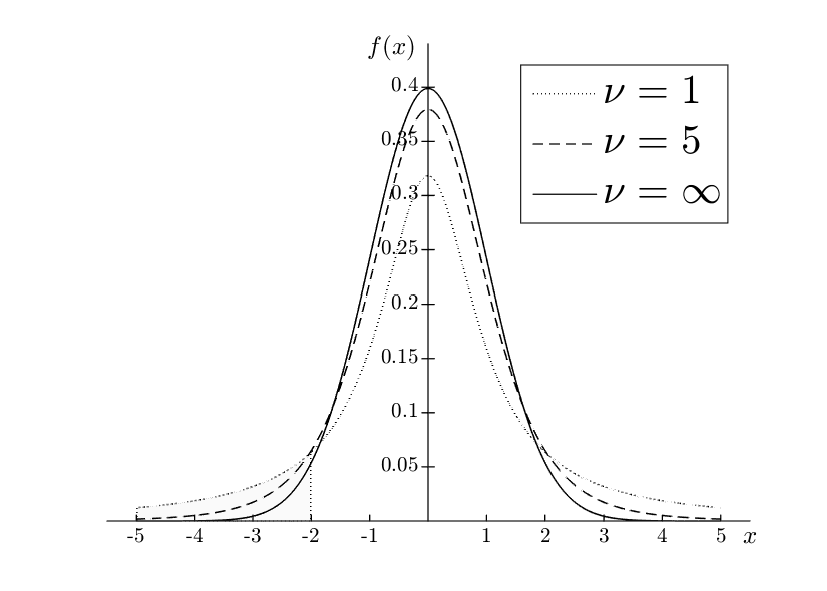
\includegraphics[scale=0.5]{img/student_pdf.png}
		\caption{Плотность вероятности}
\label{fig:a_normal_pdf}	
	\end{subfigure}
	\begin{subfigure}[t]{5cm}
		\centering
		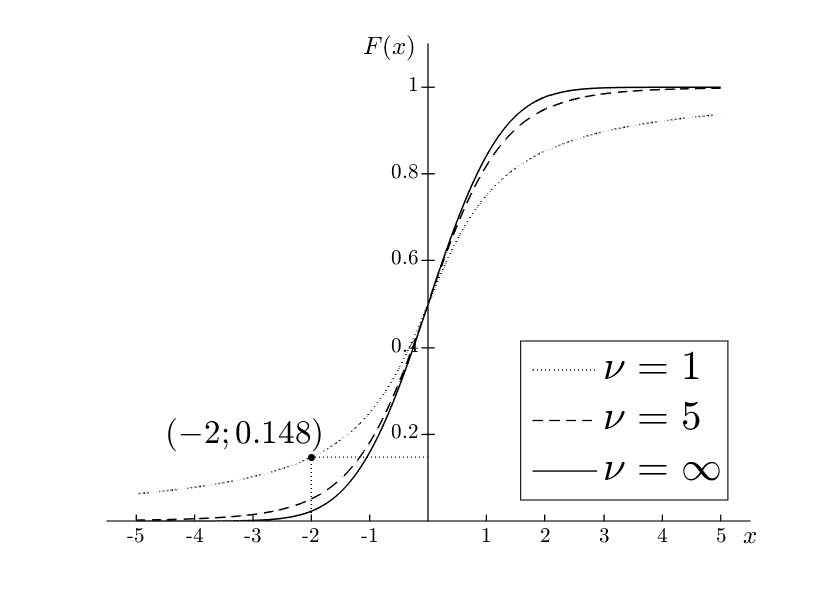
\includegraphics[scale=0.5]{img/student_cdf.png}
		\caption{Кумулятивная функция}
\label{fig:b_normal_cdf}
	\end{subfigure}
	\caption{Графики функций распределения Стьюдента}\label{fig:df_and_cdf}
\end{figure}
В силу симметричности кумулятивной функции распределения Стьюдента, значение статистики $t_{1-\alpha}$ со степенью свободы $\nu=n-1$ для квантиля $1-\alpha$ равно $-t_{\alpha}$.

% Table generated by Excel2LaTeX from sheet 'Стьюдент'
\begin{table}[htbp]
  \fontsize{10pt}{10pt}\selectfont
  \centering
  \caption{Распределение Стьюдента}
    \begin{tabular}{rrrrrrrrrrrr}
    \toprule
    $\nu$/p  & \multicolumn{1}{c}{75\%} & \multicolumn{1}{c}{77,5\%} & \multicolumn{1}{c}{80\%} & \multicolumn{1}{c}{82,5\%} & \multicolumn{1}{c}{85\%} & \multicolumn{1}{c}{87,5\%} & \multicolumn{1}{c}{90\%} & \multicolumn{1}{c}{92,5\%} & \multicolumn{1}{c}{95\%} & \multicolumn{1}{c}{97,5\%} & 99\% \\
    \midrule
    1     & 1,000 & 1,171 & 1,376 & 1,632 & 1,963 & 2,414 & 3,078 & 4,165 & 6,314 & 12,706 & 31,821 \\
    2     & 0,816 & 0,931 & 1,061 & 1,210 & 1,386 & 1,604 & 1,886 & 2,282 & 2,920 & 4,303 & 6,965 \\
    3     & 0,765 & 0,866 & 0,978 & 1,105 & 1,250 & 1,423 & 1,638 & 1,924 & 2,353 & 3,182 & 4,541 \\
    4     & 0,741 & 0,836 & 0,941 & 1,057 & 1,190 & 1,344 & 1,533 & 1,778 & 2,132 & 2,776 & 3,747 \\
    5     & 0,727 & 0,819 & 0,920 & 1,031 & 1,156 & 1,301 & 1,476 & 1,699 & 2,015 & 2,571 & 3,365 \\
    6     & 0,718 & 0,808 & 0,906 & 1,013 & 1,134 & 1,273 & 1,440 & 1,650 & 1,943 & 2,447 & 3,143 \\
    7     & 0,711 & 0,800 & 0,896 & 1,001 & 1,119 & 1,254 & 1,415 & 1,617 & 1,895 & 2,365 & 2,998 \\
    8     & 0,706 & 0,794 & 0,889 & 0,993 & 1,108 & 1,240 & 1,397 & 1,592 & 1,860 & 2,306 & 2,896 \\
    9     & 0,703 & 0,790 & 0,883 & 0,986 & 1,100 & 1,230 & 1,383 & 1,574 & 1,833 & 2,262 & 2,821 \\
    10    & 0,700 & 0,786 & 0,879 & 0,980 & 1,093 & 1,221 & 1,372 & 1,559 & 1,812 & 2,228 & 2,764 \\
    20    & 0,687 & 0,771 & 0,860 & 0,957 & 1,064 & 1,185 & 1,325 & 1,497 & 1,725 & 2,086 & 2,528 \\
    30    & 0,683 & 0,765 & 0,854 & 0,949 & 1,055 & 1,173 & 1,310 & 1,477 & 1,697 & 2,042 & 2,457 \\
    40    & 0,681 & 0,763 & 0,851 & 0,946 & 1,050 & 1,167 & 1,303 & 1,468 & 1,684 & 2,021 & 2,423 \\
    50    & 0,679 & 0,761 & 0,849 & 0,943 & 1,047 & 1,164 & 1,299 & 1,462 & 1,676 & 2,009 & 2,403 \\
    60    & 0,679 & 0,760 & 0,848 & 0,942 & 1,045 & 1,162 & 1,296 & 1,458 & 1,671 & 2,000 & 2,390 \\
    70    & 0,678 & 0,760 & 0,847 & 0,941 & 1,044 & 1,160 & 1,294 & 1,456 & 1,667 & 1,994 & 2,381 \\
    80    & 0,678 & 0,759 & 0,846 & 0,940 & 1,043 & 1,159 & 1,292 & 1,453 & 1,664 & 1,990 & 2,374 \\
    90    & 0,677 & 0,759 & 0,846 & 0,939 & 1,042 & 1,158 & 1,291 & 1,452 & 1,662 & 1,987 & 2,368 \\
    100   & 0,677 & 0,758 & 0,845 & 0,939 & 1,042 & 1,157 & 1,290 & 1,451 & 1,660 & 1,984 & 2,364 \\
    200   & 0,676 & 0,757 & 0,843 & 0,937 & 1,039 & 1,154 & 1,286 & 1,445 & 1,653 & 1,972 & 2,345 \\
    300   & 0,675 & 0,756 & 0,843 & 0,936 & 1,038 & 1,153 & 1,284 & 1,443 & 1,650 & 1,968 & 2,339 \\
    400   & 0,675 & 0,756 & 0,843 & 0,936 & 1,038 & 1,152 & 1,284 & 1,442 & 1,649 & 1,966 & 2,336 \\
    500   & 0,675 & 0,756 & 0,842 & 0,935 & 1,038 & 1,152 & 1,283 & 1,442 & 1,648 & 1,965 & 2,334 \\
    \bottomrule
    \end{tabular}%
  \label{tab:addlabel}%
\end{table}%


\textit{$\nu$} - количество степеней свободы;

\textit{p} - доверительная вероятность.

Функция \textit{Excel} СТЬЮДЕНТ.ОБР(вероятность\;степени\_свободы).
\pagebreak

\section{Распределение Фишера (F-распределение)}
\begin{figure}[H]
\centering
	\begin{subfigure}[t]{7cm}
		\centering
		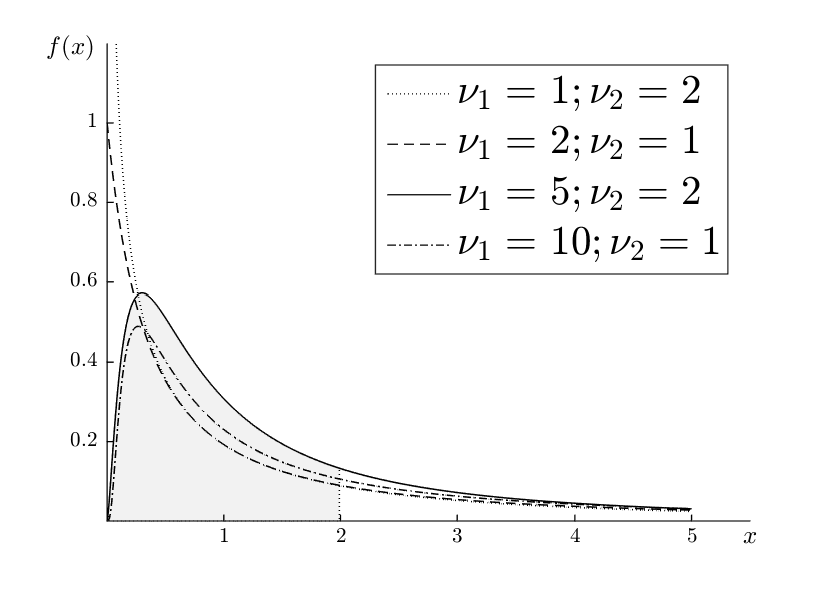
\includegraphics[scale=0.5]{img/fdistribution_pdf.png}
		\caption{Плотность вероятности}
\label{fig:a_normal_pdf}	
	\end{subfigure}
	\begin{subfigure}[t]{5cm}
		\centering
		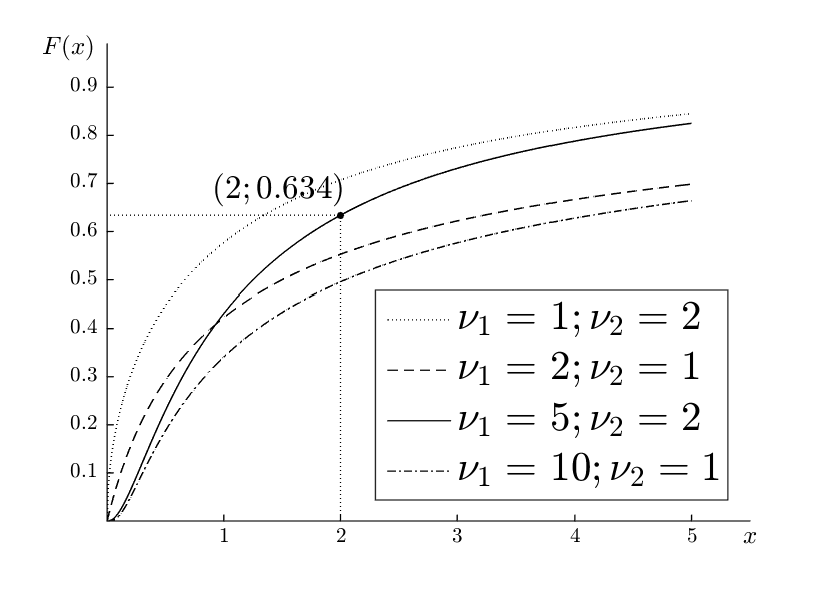
\includegraphics[scale=0.5]{img/fdistribution_cdf.png}
		\caption{Кумулятивная функция}
\label{fig:b_normal_cdf}
	\end{subfigure}
	\caption{Графики функций F-распределения}\label{fig:df_and_cdf}
\end{figure}
% Table generated by Excel2LaTeX from sheet 'фишер'
\begin{table}[htbp]
  \centering
  \caption{F-распределение, $\alpha=5\%$}
    \begin{tabular}{crrrrrrrrrr}
    \toprule
    $\nu_2/\nu_1$  & \multicolumn{1}{c}{           10   } & \multicolumn{1}{c}{           20   } & \multicolumn{1}{c}{           30   } & \multicolumn{1}{c}{           40   } & \multicolumn{1}{c}{           50   } & \multicolumn{1}{c}{           60   } & \multicolumn{1}{c}{           70   } & \multicolumn{1}{c}{           80   } & \multicolumn{1}{c}{           90   } & \multicolumn{1}{c}{         100   } \\
    \midrule
    10    & 2,978 & 2,774 & 2,700 & 2,661 & 2,637 & 2,621 & 2,610 & 2,601 & 2,594 & 2,588 \\
    20    & 2,348 & 2,124 & 2,039 & 1,994 & 1,966 & 1,946 & 1,932 & 1,922 & 1,913 & 1,907 \\
    30    & 2,165 & 1,932 & 1,841 & 1,792 & 1,761 & 1,740 & 1,724 & 1,712 & 1,703 & 1,695 \\
    40    & 2,077 & 1,839 & 1,744 & 1,693 & 1,660 & 1,637 & 1,621 & 1,608 & 1,597 & 1,589 \\
    50    & 2,026 & 1,784 & 1,687 & 1,634 & 1,599 & 1,576 & 1,558 & 1,544 & 1,534 & 1,525 \\
    60    & 1,993 & 1,748 & 1,649 & 1,594 & 1,559 & 1,534 & 1,516 & 1,502 & 1,491 & 1,481 \\
    70    & 1,969 & 1,722 & 1,622 & 1,566 & 1,530 & 1,505 & 1,486 & 1,471 & 1,459 & 1,450 \\
    80    & 1,951 & 1,703 & 1,602 & 1,545 & 1,508 & 1,482 & 1,463 & 1,448 & 1,436 & 1,426 \\
    90    & 1,938 & 1,688 & 1,586 & 1,528 & 1,491 & 1,465 & 1,445 & 1,429 & 1,417 & 1,407 \\
    100   & 1,927 & 1,676 & 1,573 & 1,515 & 1,477 & 1,450 & 1,430 & 1,415 & 1,402 & 1,392 \\
    \bottomrule
    \end{tabular}%
  \label{tab:addlabel}%
\end{table}%
% Table generated by Excel2LaTeX from sheet 'фишер'
\begin{table}[htbp]
  \centering
  \caption{F-распределение, $\alpha=10\%$}
    \begin{tabular}{crrrrrrrrrr}
    \toprule
    $\nu_2/\nu_1$  & \multicolumn{1}{c}{           10   } & \multicolumn{1}{c}{           20   } & \multicolumn{1}{c}{           30   } & \multicolumn{1}{c}{           40   } & \multicolumn{1}{c}{           50   } & \multicolumn{1}{c}{           60   } & \multicolumn{1}{c}{           70   } & \multicolumn{1}{c}{           80   } & \multicolumn{1}{c}{           90   } & \multicolumn{1}{c}{         100   } \\
    \midrule
    10    & 2,323 & 2,201 & 2,155 & 2,132 & 2,117 & 2,107 & 2,100 & 2,095 & 2,090 & 2,087 \\
    20    & 1,937 & 1,794 & 1,738 & 1,708 & 1,690 & 1,677 & 1,667 & 1,660 & 1,655 & 1,650 \\
    30    & 1,819 & 1,667 & 1,606 & 1,573 & 1,552 & 1,538 & 1,527 & 1,519 & 1,512 & 1,507 \\
    40    & 1,763 & 1,605 & 1,541 & 1,506 & 1,483 & 1,467 & 1,455 & 1,447 & 1,439 & 1,434 \\
    50    & 1,729 & 1,568 & 1,502 & 1,465 & 1,441 & 1,424 & 1,412 & 1,402 & 1,395 & 1,388 \\
    60    & 1,707 & 1,543 & 1,476 & 1,437 & 1,413 & 1,395 & 1,382 & 1,372 & 1,364 & 1,358 \\
    70    & 1,691 & 1,526 & 1,457 & 1,418 & 1,392 & 1,374 & 1,361 & 1,350 & 1,342 & 1,335 \\
    80    & 1,680 & 1,513 & 1,443 & 1,403 & 1,377 & 1,358 & 1,344 & 1,334 & 1,325 & 1,318 \\
    90    & 1,670 & 1,503 & 1,432 & 1,391 & 1,365 & 1,346 & 1,332 & 1,321 & 1,312 & 1,304 \\
    100   & 1,663 & 1,494 & 1,423 & 1,382 & 1,355 & 1,336 & 1,321 & 1,310 & 1,301 & 1,293 \\
    \bottomrule
    \end{tabular}%
  \label{tab:addlabel}%
\end{table}%
\textit{$\nu_1,\nu_2$} - количество степеней свободы;

Функция \textit{Excel} F.ОБР(вероятность\;степени\_свободы1\;степени\_свободы2).
\pagebreak

\section{Распределение хи-квадрат}
\begin{figure}[H]
\centering
	\begin{subfigure}[t]{7cm}
		\centering
		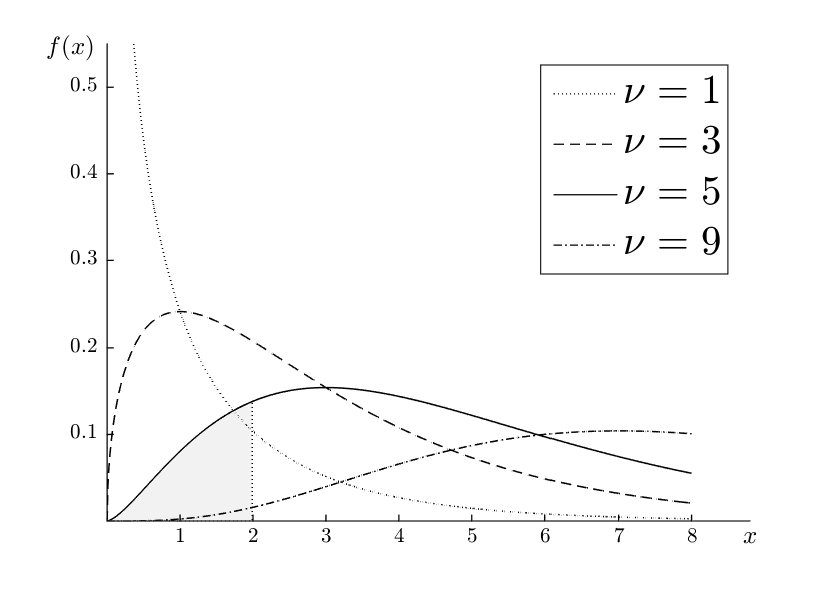
\includegraphics[scale=0.5]{img/xdistribution_pdf.png}
		\caption{Плотность вероятности}
\label{fig:a_normal_pdf}	
	\end{subfigure}
	\begin{subfigure}[t]{5cm}
		\centering
		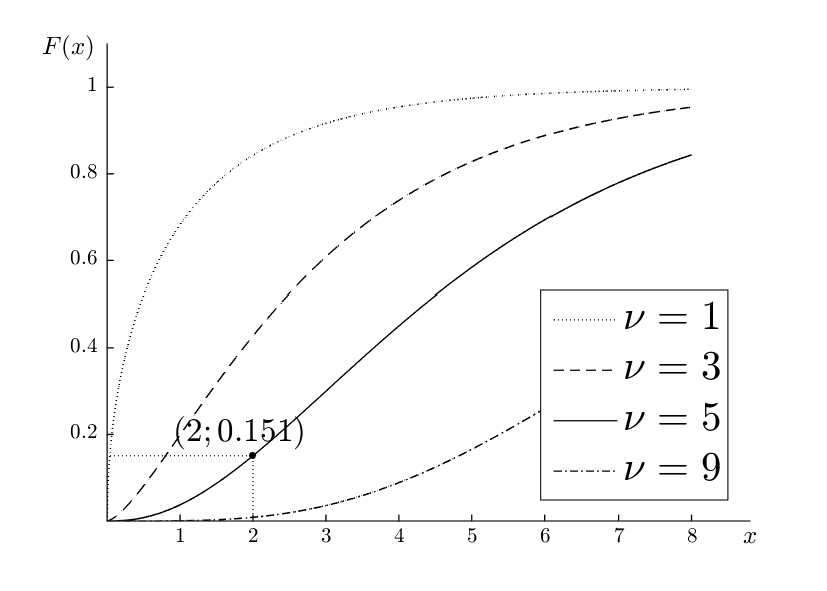
\includegraphics[scale=0.5]{img/xdistribution_cdf.png}
		\caption{Кумулятивная функция}
\label{fig:b_normal_cdf}
	\end{subfigure}
	\caption{Графики функций распределения $\chi^2$ (хи-квадрат)}\label{fig:df_and_cdf}
\end{figure}
% Table generated by Excel2LaTeX from sheet 'хи-квадрат'
\begin{table}[htbp]
  \centering
  \caption{Распределение хи-квадрат}
    \begin{tabular}{crrrrrrrrrr}
    \toprule
    $\nu$/p  & \multicolumn{1}{c}{0,50\%} & \multicolumn{1}{c}{1\%} & \multicolumn{1}{c}{2,50\%} & \multicolumn{1}{c}{5\%} & \multicolumn{1}{c}{10\%} & \multicolumn{1}{c}{90\%} & \multicolumn{1}{c}{95\%} & \multicolumn{1}{c}{97,50\%} & \multicolumn{1}{c}{99\%} & \multicolumn{1}{c}{99,50\%} \\
    \midrule
    10    & 2,16  & 2,56  & 3,25  & 3,94  & 4,87  & 15,99 & 18,31 & 20,48 & 23,21 & 25,19 \\
    20    & 7,43  & 8,26  & 9,59  & 10,85 & 12,44 & 28,41 & 31,41 & 34,17 & 37,57 & 40,00 \\
    30    & 13,79 & 14,95 & 16,79 & 18,49 & 20,60 & 40,26 & 43,77 & 46,98 & 50,89 & 53,67 \\
    40    & 20,71 & 22,16 & 24,43 & 26,51 & 29,05 & 51,81 & 55,76 & 59,34 & 63,69 & 66,77 \\
    50    & 27,99 & 29,71 & 32,36 & 34,76 & 37,69 & 63,17 & 67,50 & 71,42 & 76,15 & 79,49 \\
    60    & 35,53 & 37,48 & 40,48 & 43,19 & 46,46 & 74,40 & 79,08 & 83,30 & 88,38 & 91,95 \\
    70    & 43,28 & 45,44 & 48,76 & 51,74 & 55,33 & 85,53 & 90,53 & 95,02 & 100,43 & 104,21 \\
    80    & 51,17 & 53,54 & 57,15 & 60,39 & 64,28 & 96,58 & 101,88 & 106,63 & 112,33 & 116,32 \\
    90    & 59,20 & 61,75 & 65,65 & 69,13 & 73,29 & 107,57 & 113,15 & 118,14 & 124,12 & 128,30 \\
    100   & 67,33 & 70,06 & 74,22 & 77,93 & 82,36 & 118,50 & 124,34 & 129,56 & 135,81 & 140,17 \\
    125   & 88,03 & 91,18 & 95,95 & 100,18 & 105,21 & 145,64 & 152,09 & 157,84 & 164,69 & 169,47 \\
    150   & 109,14 & 112,67 & 117,98 & 122,69 & 128,28 & 172,58 & 179,58 & 185,80 & 193,21 & 198,36 \\
    175   & 130,57 & 134,44 & 140,26 & 145,41 & 151,49 & 199,36 & 206,87 & 213,52 & 221,44 & 226,94 \\
    200   & 152,24 & 156,43 & 162,73 & 168,28 & 174,84 & 226,02 & 233,99 & 241,06 & 249,45 & 255,26 \\
    225   & 174,12 & 178,61 & 185,35 & 191,28 & 198,28 & 252,58 & 260,99 & 268,44 & 277,27 & 283,39 \\
    250   & 196,16 & 200,94 & 208,10 & 214,39 & 221,81 & 279,05 & 287,88 & 295,69 & 304,94 & 311,35 \\
    275   & 218,35 & 223,40 & 230,96 & 237,59 & 245,41 & 305,45 & 314,68 & 322,83 & 332,48 & 339,16 \\
    300   & 240,66 & 245,97 & 253,91 & 260,88 & 269,07 & 331,79 & 341,40 & 349,87 & 359,91 & 366,84 \\
    \bottomrule
    \end{tabular}%
  \label{tab:addlabel}%
\end{table}%

\textit{$\nu$} - количество степеней свободы;

\textit{p} - доверительная вероятность.

Функция \textit{Excel} ХИ2.ОБР(вероятность;степени\_свободы).

\end{document}